\documentclass[12pt,a4paper]{report}

% ─────────────────────── PACKAGES ───────────────────────
\usepackage[margin=2.5cm]{geometry}
\usepackage{amsmath, amssymb, amsthm}
\usepackage{graphicx}
\usepackage{float}
\usepackage{booktabs}
\usepackage{longtable}
\usepackage{hyperref}
\usepackage{listings}
\usepackage{xcolor}
\usepackage{array}
\usepackage{enumitem}
\usepackage{fancyhdr}
\usepackage{titlesec}
\usepackage{caption}
\usepackage{subcaption}
\usepackage{algorithm}
\usepackage{algpseudocode}
\usepackage{cite}
\usepackage{url}

% ─────────────────────── STYLING ───────────────────────
\hypersetup{
    colorlinks=true, linkcolor=blue, citecolor=blue, urlcolor=blue
}
\pagestyle{fancy}
\fancyhf{}
\fancyhead[L]{\small FedGen-Rare: SDP Review 2 Report}
\fancyhead[R]{\small Dept. of Computer Science and Engineering}
\fancyfoot[C]{\thepage}
\renewcommand{\headrulewidth}{0.4pt}

% Code listing style
\lstset{
    basicstyle=\small\ttfamily,
    keywordstyle=\bfseries\color{blue},
    commentstyle=\itshape\color{gray},
    stringstyle=\color{red!70!black},
    numbers=left, numberstyle=\tiny\color{gray},
    frame=single, breaklines=true, showstringspaces=false,
    language=Python
}

% ─────────────────────── TITLE PAGE ───────────────────────
\begin{document}

\begin{titlepage}
    \centering
    \vspace{2cm}
    {\Large \textbf{Department of Computer Science and Engineering}}\\[0.4cm]
    {\large \textit{KLE Technological University, Hubballi}}\\[2cm]

    \rule{\linewidth}{0.5mm}\\[0.5cm]
    {\LARGE \bfseries FedGen-Rare: Privacy-Preserving Federated\\[0.3cm]
    Generative Replay for Rare Disease Diagnosis}\\[0.3cm]
    {\large A Multi-Center Study on Idiopathic Pulmonary Fibrosis (IPF)}\\[0.3cm]
    \rule{\linewidth}{0.5mm}\\[1.5cm]

    \textbf{Senior Design Project (SDP) — Review 2 Report}\\
    \textbf{Course Code:} 22ECAW401 \quad \textbf{Semester:} 07 \quad \textbf{Year:} 2026-27\\[2cm]

    \begin{tabular}{ll}
        \textbf{Team Members:} & Ishwari J (01FE22BCS135)\\
                               & Rakshita J (01FE22BCS184)\\
                               & Amrutavarshini B (01FE22BCS016)\\
                               & Aditya C (01FE22BCS004)\\[0.5cm]
        \textbf{Project Guide:} & Prof. Mallikarjun Akki\\[0.5cm]
        \textbf{GitHub:} & \url{https://github.com/Aditya-c-hu/}\\
                         & \url{FedGen-Rare-for-Idiopathic-Pulmonary-Fibrosis}
    \end{tabular}

    \vfill
    {\large \today}
\end{titlepage}

% ─────────────────────── TABLE OF CONTENTS ───────────────────────
\tableofcontents
\listoffigures
\listoftables
\newpage

% ─────────────────────── ABSTRACT ───────────────────────
\chapter*{Abstract}
\addcontentsline{toc}{chapter}{Abstract}

Idiopathic Pulmonary Fibrosis (IPF, ORPHA:2032) is an ultra-rare, progressive, and fatal fibrotic interstitial lung disease with a median post-diagnosis survival of 2 to 3 years. Early and accurate diagnosis is critically obstructed by its extreme rarity ($<$8\% prevalence in pulmonary cohorts), visual similarity to common Chronic Obstructive Pulmonary Disease (COPD) and Interstitial Lung Disease (ILD) on High-Resolution Computed Tomography (HRCT) imaging, and strict patient data privacy regulations (HIPAA/GDPR) that prohibit centralizing raw patient scans across hospital boundaries.

This report presents \textbf{FedGen-Rare}, a novel privacy-preserving federated learning framework that addresses the fundamental limitation of state-of-the-art methods like FedIIC (MICCAI 2023): their mathematical inability to handle hospital clients with zero or only one patient case of the rare target disease. FedGen-Rare introduces a \textbf{Two-Stage Federated Latent Generative Replay} pipeline. A conditional feature generator $\mathcal{G}_\psi$ is collaboratively trained across hospital nodes and used to synthesize privacy-safe latent feature representations of IPF, rebalancing local optimization without transmitting any patient scan pixels.

Benchmarked against FedAvg, FedProx, and FedIIC on a realistic multi-center non-IID HRCT cohort with Dirichlet skew ($\alpha=0.2$), FedGen-Rare achieves a \textbf{+28.6\% improvement in rare disease sensitivity (IPF Recall)} and a \textbf{+18.3\% improvement in Balanced Accuracy} over the MICCAI '23 state-of-the-art.

\newpage

% ─────────────────────── CHAPTER 1: SYSTEM REQUIREMENTS ───────────────────────
\chapter{System Requirements}
\label{ch:requirements}

\section{Problem Statement}
The core problem is designing a federated learning system that can accurately detect Idiopathic Pulmonary Fibrosis (IPF) from Chest HRCT scans across multiple hospital silos, where:
\begin{itemize}
    \item Hospitals cannot share raw patient scan data due to privacy regulations.
    \item IPF is rare — most hospitals observe fewer than 5 IPF cases per year.
    \item Standard federated averaging methods suffer from complete recall collapse on the rare IPF class.
\end{itemize}

\section{Design Principles}
The following design principles were selected and justified for developing FedGen-Rare:

\begin{enumerate}
    \item \textbf{Privacy-by-Design (Federated Learning):} Raw CT pixel data never leaves hospital premises. Only model gradient updates (weights) and latent feature distributions are communicated.
    \item \textbf{Class-Imbalance Awareness:} System must explicitly handle minority class (IPF $\approx8\%$) via generative rebalancing rather than standard uniform loss.
    \item \textbf{Client-Agnostic Generalization:} The framework must function even for hospital clients with zero examples of the rare class, unlike contrastive methods requiring positive pairs.
    \item \textbf{Modularity (Strategy Pattern):} Federated training algorithms (FedAvg, FedProx, FedIIC, FedGen-Rare) are swappable without modifying server/client interfaces.
\end{enumerate}

\section{Functional Requirements}
\begin{longtable}{|p{0.5cm}|p{5cm}|p{8cm}|}
    \hline
    \textbf{FR\#} & \textbf{Requirement} & \textbf{Description} \\
    \hline
    FR1 & Multi-Center Data Partitioning & System must partition a global dataset across hospital silos using Dirichlet distribution ($\alpha=0.2$) to simulate real-world non-IID clinical scarcity. \\
    \hline
    FR2 & Local Classifier Training & Each hospital client must be capable of training a local diagnostic classifier using its private HRCT data and a locally deployed feature generator. \\
    \hline
    FR3 & Federated Generator Distillation & Each hospital client must train a local conditional feature generator $\mathcal{G}_\psi$ using knowledge distilled from the global diagnostic classifier. \\
    \hline
    FR4 & Generative Replay Rebalancing & During classifier training, if a hospital's local batch contains fewer IPF samples than the target, the system must synthesize synthetic IPF latent features $\hat{f}_\text{IPF}$ to rebalance training. \\
    \hline
    FR5 & Federated Aggregation & Server must aggregate both generator weights $\psi$ and classifier weights $\theta$ from all clients via weighted FedAvg. \\
    \hline
    FR6 & Baseline Comparison & System must support FedAvg, FedProx, and FedIIC in addition to FedGen-Rare for 4-way comparative benchmarking. \\
    \hline
    FR7 & Global Evaluation & After each round, the global classifier must be evaluated on a held-out test set reporting BACC, IPF Recall, IPF F1, Macro-F1, and AUROC. \\
    \hline
    FR8 & Visualization & Benchmark outputs must include comparative bar charts, client distribution plots, and confusion matrices. \\
    \hline
\end{longtable}

\section{Non-Functional Requirements}
\begin{longtable}{|p{0.5cm}|p{4cm}|p{9cm}|}
    \hline
    \textbf{NFR\#} & \textbf{Requirement} & \textbf{Description} \\
    \hline
    NFR1 & Privacy & Zero raw HRCT pixel data leaves hospital premises. Only 128-dimensional latent vectors are shared. \\
    \hline
    NFR2 & Scalability & System must support 3 to 20 hospital client nodes without code changes. \\
    \hline
    NFR3 & Reproducibility & Full benchmark must be reproducible with a single seed parameter ($\text{seed}=42$). \\
    \hline
    NFR4 & Portability & Code must run on any Python 3.10+ system with PyTorch, whether CPU-only or GPU-enabled. \\
    \hline
    NFR5 & Maintainability & Each federated algorithm (FedAvg, FedGen-Rare, etc.) must be modifiable independently without affecting others. \\
    \hline
    NFR6 & Performance (Speed) & A 3-round quick-test benchmark across 3 clients must complete within 3 minutes on a standard CPU. \\
    \hline
\end{longtable}

\section{Constraints and Assumptions}
\textbf{Constraints:}
\begin{itemize}
    \item Benchmark is performed on synthetic HRCT data simulating realistic CT physics (no access to actual patient DICOM data due to HIPAA).
    \item All computation is performed on CPU (no GPU requirement for baseline runs).
    \item Number of classes is fixed at 3 (IPF, Common ILD/COPD, Normal).
\end{itemize}

\textbf{Assumptions:}
\begin{itemize}
    \item Communication channels between hospital nodes and the server are reliable and synchronous within each federated round.
    \item All hospitals use compatible image preprocessing pipelines (64$\times$64 HRCT slice normalization).
    \item The federated server is a trusted aggregator (honest-but-curious threat model).
\end{itemize}

\newpage

% ─────────────────────── CHAPTER 2: ARCHITECTURAL FRAMEWORK ───────────────────────
\chapter{Architectural Framework and Design Principles}
\label{ch:architecture}

\section{System Architecture Overview}

FedGen-Rare adopts a \textbf{hierarchical federated client-server architecture} augmented with a conditional latent feature generator for privacy-safe data augmentation.

\begin{figure}[H]
    \centering
    % \includegraphics[width=\linewidth]{../uml/component_diagram.png}
    \caption{FedGen-Rare System Component Architecture. The global server maintains $\mathcal{F}_\theta$ and $\mathcal{G}_\psi$; hospital clients perform local generative replay before uploading weight updates.}
    \label{fig:component}
\end{figure}

\section{Design Patterns Applied}

\subsection{Strategy Pattern (Federated Algorithm Selection)}
The \texttt{FederatedServer} class exposes a clean interface for swapping between four federated training algorithms:
\begin{itemize}
    \item \texttt{train\_round\_fedavg()} — McMahan et al. (2017)
    \item \texttt{train\_round\_fedprox()} — Li et al. (2020)
    \item \texttt{train\_round\_fediic()} — Wu et al. (MICCAI 2023)
    \item \texttt{train\_round\_fedgen\_rare()} — Proposed
\end{itemize}
This \textbf{Strategy Pattern} enables algorithm replacement without modifying client or server internals, satisfying NFR5 (Maintainability).

\subsection{Producer-Consumer Pattern (Generative Replay)}
The conditional feature generator $\mathcal{G}_\psi$ acts as a \textbf{producer} of synthetic rare-class feature vectors, while the local classifier training loop acts as the \textbf{consumer}. This decoupling ensures privacy (the producer never sees raw patient images) and modularity.

\subsection{Factory Pattern (Classifier Construction)}
The \texttt{build\_classifier(backbone)} factory function abstracts backbone selection (ConvNet or ResNet-18) from the rest of the system, allowing backbone upgrades without modifying training logic.

\section{Design Criteria for Solution Selection}

The following criteria were used to justify the architectural choices:

\begin{table}[H]
    \centering
    \caption{Design Decision Matrix: Selection Criteria and Justification}
    \label{tab:design_decision}
    \begin{tabular}{|p{4cm}|p{4cm}|p{6cm}|}
        \hline
        \textbf{Design Dimension} & \textbf{Alternative Considered} & \textbf{Chosen Solution \& Justification} \\
        \hline
        Image-space generation & GAN on raw CT images & \textbf{Latent feature generation:} avoids unstable GAN training, 100$\times$ smaller models, no pixel data leakage. \\
        \hline
        Aggregation & Weighted FedMA, FedBN & \textbf{Weighted FedAvg:} simpler, proven reliable, compatible with both generator and classifier. \\
        \hline
        Backbone & VGG-16, EfficientNet & \textbf{ConvNet / ResNet-18:} lightweight for CPU hospital edge nodes; sufficient for 64$\times$64 HRCT slices. \\
        \hline
        Class rebalancing & Over-sampling, SMOTE & \textbf{Generative replay:} operates in latent space, is privacy-safe, does not require raw image access. \\
        \hline
    \end{tabular}
\end{table}

\section{UML Diagrams}

\subsection{Class Diagram}
Refer to \texttt{docs/uml/02\_class\_diagram.puml}. This diagram shows the full class hierarchy:
\begin{itemize}
    \item \texttt{BaseClassifier} $\leftarrow$ \texttt{ConvNet}, \texttt{ResNetClassifier}
    \item \texttt{HospitalClient} aggregates \texttt{IPFChestCTDataset} and uses \texttt{DeviceAgnosticDALA}, \texttt{ContrastiveAlignmentLoss}
    \item \texttt{FederatedServer} orchestrates \texttt{HospitalClient} list and maintains global models
\end{itemize}

\subsection{Sequence Diagram}
Refer to \texttt{docs/uml/03\_sequence\_diagram.puml}. Key flows:
\begin{enumerate}
    \item Server distributes $\theta, \psi$ to all hospital clients.
    \item Each hospital trains a local generator copy (Stage 1).
    \item Updated generators are aggregated via FedAvg.
    \item Each hospital trains the classifier using generative replay (Stage 2).
    \item Updated classifiers are aggregated via FedAvg.
    \item Global evaluation is performed on the held-out test set.
\end{enumerate}

\newpage

% ─────────────────────── CHAPTER 3: DETAILED DESIGN ───────────────────────
\chapter{Detailed Design}
\label{ch:design}

\section{Mathematical Formulations}

\subsection{Problem Formulation}
Let $K$ denote the number of hospital silos (clients). Hospital $k$ holds private dataset $\mathcal{D}_k = \{(x_i, y_i)\}_{i=1}^{n_k}$ where $y_i \in \{0, 1, 2\}$ (IPF, COPD, Normal). The global federated objective is:
\begin{equation}
    \min_{\theta} \; \mathcal{F}(\theta) = \sum_{k=1}^{K} \frac{n_k}{N} \mathcal{F}_k(\theta), \quad N = \sum_k n_k
    \label{eq:global_obj}
\end{equation}
However, under Dirichlet non-IID skew ($\alpha=0.2$), many clients have $n_k^{(\text{IPF})} \in \{0, 1\}$, causing standard FedAvg to suffer rare-class gradient starvation.

\subsection{Conditional Latent Feature Generator $\mathcal{G}_\psi$}
Instead of generating raw CT images (unstable, high-dimensional), $\mathcal{G}_\psi$ generates 128-dimensional latent feature vectors conditioned on class label $y$:
\begin{equation}
    \hat{f} = \mathcal{G}_\psi(z, y), \quad z \sim \mathcal{N}(0, I_{d_z}), \quad y \in \{0, 1, \ldots, C-1\}
    \label{eq:gen_forward}
\end{equation}

\subsection{Generator Training Objective}
The local generator at hospital $k$ is trained to minimize three complementary losses:
\begin{equation}
    \mathcal{L}_{\text{gen}} = \underbrace{\mathcal{L}_{\text{CE}}(\mathcal{F}_\theta(\hat{f}), y)}_{\text{Classification Fidelity}} + \underbrace{\lambda_{\text{fm}} \cdot \mathcal{L}_{\text{FM}}(\hat{f}, \bar{f}_c^k)}_{\text{Feature Matching}} - \underbrace{\lambda_{\text{div}} \cdot \frac{\|\hat{f}_1 - \hat{f}_2\|_1}{\|z_1 - z_2\|_1 + \epsilon}}_{\text{Mode-Seeking Diversity}}
    \label{eq:gen_loss}
\end{equation}
where:
\begin{itemize}
    \item $\mathcal{L}_{\text{FM}}(\hat{f}, \bar{f}_c^k) = \text{MSE}\!\left(\mathbb{E}_{c}[\hat{f}], \bar{f}_c^k\right)$ grounds synthetic features in real local clinical representations.
    \item The diversity term prevents mode collapse by penalizing identical outputs for different noise inputs.
\end{itemize}

\subsection{Generative Replay Classifier Training}
During classifier training, for each client batch, synthetic rare-class features are appended to rebalance the effective class distribution:
\begin{equation}
    f_{\text{combined}} = \text{Concat}\!\left[f_{\text{real}}, \hat{f}_{\text{IPF}}\right], \quad
    y_{\text{combined}} = \text{Concat}\!\left[y_{\text{real}}, \mathbf{y}_\text{IPF}\right]
    \label{eq:replay}
\end{equation}
\begin{equation}
    \mathcal{L}_{\text{clf}} = \mathcal{L}_{\text{CE}}\!\left(\text{ClassifierHead}(f_{\text{combined}}), \; y_{\text{combined}}\right)
    \label{eq:clf_loss}
\end{equation}

\subsection{Why FedIIC Fails on Rare Diseases}
FedIIC's \textbf{IntraSCL} contrastive loss requires at least two samples of the same class ($|P(i)| \geq 1$):
\begin{equation}
    \mathcal{L}_{\text{IntraSCL}} = -\sum_{i \in I} \frac{1}{|P(i)|} \sum_{p \in P(i)} \log \frac{\exp(z_i \cdot z_p / \tau)}{\sum_{a \in A(i)} \exp(z_i \cdot z_a / \tau)}
    \label{eq:fediic_scl}
\end{equation}
When a hospital has $n_k^{(\text{IPF})} = 0$ or $1$, $|P(i)| = 0$ for IPF, causing complete contrastive alignment failure for the rare class.

\section{Algorithms and Pseudocode}

\subsection{Algorithm 1: Local Generator Distillation}

\begin{algorithm}[H]
\caption{Local Generator Training with Feature Matching (Hospital $k$)}
\label{alg:gen_train}
\begin{algorithmic}[1]
\Require Local dataset $\mathcal{D}_k$, global classifier $\mathcal{F}_\theta$, global generator $\mathcal{G}_\psi$, steps $T$, $\lambda_{\text{fm}}$, $\lambda_{\text{div}}$
\Ensure Updated local generator weights $\psi_k$
\State $\mathcal{G}_\psi \leftarrow \text{copy}(\mathcal{G}_\psi^{\text{global}})$
\State \textbf{Compute real feature centroids:}
\For{each batch $(x, y)$ in $\mathcal{D}_k$}
    \State $f \leftarrow \mathcal{F}_\theta.\text{extract\_features}(x)$
    \For{each class $c \in \{0,\ldots,C-1\}$} \textbf{with} $y = c$
        \State $\bar{f}_c^k \leftarrow \text{mean}(f[y = c])$
    \EndFor
\EndFor
\For{$t = 1$ to $T$}
    \State Sample $z \sim \mathcal{N}(0, I)$, sample target labels $\hat{y}$ (50\% IPF, 50\% uniform)
    \State $\hat{f} \leftarrow \mathcal{G}_\psi(z, \hat{y})$
    \State $\mathcal{L}_{\text{CE}} \leftarrow \text{CrossEntropy}(\mathcal{F}_\theta(\hat{f}), \hat{y})$
    \State $\mathcal{L}_{\text{FM}} \leftarrow \frac{1}{|C_k|}\sum_{c \in C_k} \text{MSE}(\text{mean}(\hat{f}[\hat{y}=c]),\, \bar{f}_c^k)$
    \State $\mathcal{L}_{\text{div}} \leftarrow -\|\hat{f}_1 - \hat{f}_2\|_1 / (\|z_1 - z_2\|_1 + \epsilon)$
    \State $\mathcal{L}_{\text{gen}} \leftarrow \mathcal{L}_{\text{CE}} + \lambda_{\text{fm}} \cdot \mathcal{L}_{\text{FM}} + \lambda_{\text{div}} \cdot \mathcal{L}_{\text{div}}$
    \State $\psi_k \leftarrow \psi_k - \eta_g \nabla_\psi \mathcal{L}_{\text{gen}}$
\EndFor
\State \Return $\psi_k$
\end{algorithmic}
\end{algorithm}

\subsection{Algorithm 2: Classifier Training with Generative Replay}

\begin{algorithm}[H]
\caption{Local Classifier Training via Generative Replay (Hospital $k$)}
\label{alg:clf_replay}
\begin{algorithmic}[1]
\Require Local dataset $\mathcal{D}_k$, global generator $\mathcal{G}_\psi$, local classifier copy $\mathcal{F}_\theta^k$, local epochs $E$, rare class index $r$, batch size $B$
\Ensure Updated classifier weights $\theta_k$
\For{epoch $e = 1$ to $E$}
    \For{each batch $(x, y)$ in $\mathcal{D}_k$}
        \State $f_{\text{real}} \leftarrow \mathcal{F}_\theta^k.\text{extract\_features}(x)$
        \State $n_{\text{rare}} \leftarrow |\{i : y_i = r\}|$
        \State $n_{\text{syn}} \leftarrow \max\!\left(2,\, \lfloor B/C \rfloor - n_{\text{rare}}\right)$
        \If{$n_{\text{syn}} > 0$}
            \State $\hat{y}_{\text{syn}} \leftarrow [r] \times n_{\text{syn}}$
            \State $\hat{f}_{\text{syn}} \leftarrow \mathcal{G}_\psi.\text{sample}(\hat{y}_{\text{syn}})$
            \State $f_{\text{comb}} \leftarrow \text{Concat}[f_{\text{real}},\, \hat{f}_{\text{syn}}]$
            \State $y_{\text{comb}} \leftarrow \text{Concat}[y,\, \hat{y}_{\text{syn}}]$
        \Else
            \State $f_{\text{comb}}, y_{\text{comb}} \leftarrow f_{\text{real}}, y$
        \EndIf
        \State $\mathcal{L}_{\text{clf}} \leftarrow \text{CrossEntropy}(\mathcal{F}_\theta^k.\text{forward\_head}(f_{\text{comb}}),\, y_{\text{comb}})$
        \State $\theta_k \leftarrow \theta_k - \eta_c \nabla_\theta \mathcal{L}_{\text{clf}}$
    \EndFor
\EndFor
\State \Return $\theta_k$
\end{algorithmic}
\end{algorithm}

\subsection{Algorithm 3: FedGen-Rare Global Round}

\begin{algorithm}[H]
\caption{FedGen-Rare: Full Global Communication Round (Server)}
\label{alg:fedgen_rare_round}
\begin{algorithmic}[1]
\Require Hospital clients $\{C_1, \ldots, C_K\}$, global classifier $\mathcal{F}_\theta$, global generator $\mathcal{G}_\psi$, client weights $\{w_k = n_k/N\}$
\Ensure Updated $\mathcal{F}_\theta$, $\mathcal{G}_\psi$
\State \textbf{// Stage 1: Federated Generator Update}
\State Broadcast $(\theta_{\text{global}}, \psi_{\text{global}})$ to all $K$ hospitals
\For{each hospital $k = 1$ to $K$}
    \State $\psi_k \leftarrow \textsc{LocalGenTrain}(\mathcal{D}_k, \mathcal{F}_{\theta_\text{global}}, \mathcal{G}_{\psi_\text{global}}, T=5)$ \Comment{Algorithm 1}
\EndFor
\State $\psi_{\text{global}} \leftarrow \sum_k w_k \cdot \psi_k$ \Comment{FedAvg generator aggregation}
\State $\mathcal{G}_\psi.\text{load}(\psi_{\text{global}})$

\State \textbf{// Stage 2: Federated Classifier Update with Replay}
\For{each hospital $k = 1$ to $K$}
    \State $\theta_k \leftarrow \textsc{ClfReplayTrain}(\mathcal{D}_k, \mathcal{G}_{\psi_\text{global}}, \mathcal{F}_\theta^k, E)$ \Comment{Algorithm 2}
\EndFor
\State $\theta_{\text{global}} \leftarrow \sum_k w_k \cdot \theta_k$ \Comment{FedAvg classifier aggregation}
\State $\mathcal{F}_\theta.\text{load}(\theta_{\text{global}})$
\State \Return $(\mathcal{F}_\theta, \mathcal{G}_\psi)$
\end{algorithmic}
\end{algorithm}

\newpage

% ─────────────────────── CHAPTER 4: TOOLS & TECHNOLOGIES ───────────────────────
\chapter{Modern Tools and Techniques}
\label{ch:tools}

\section{Development Environment}
\begin{table}[H]
    \centering
    \caption{Development Tools and Technologies Used}
    \label{tab:tools}
    \begin{tabular}{|p{3.5cm}|p{3.5cm}|p{7cm}|}
        \hline
        \textbf{Tool / Technology} & \textbf{Version} & \textbf{Purpose and Justification} \\
        \hline
        Python & 3.13 & Primary implementation language. Object-oriented programming paradigm. \\
        \hline
        PyTorch & 2.14.1 & Deep learning framework for CNN models, gradient computation, and CUDA/CPU portability. \\
        \hline
        Torchvision & 0.29.1 & ResNet-18 backbone and standard image transforms. \\
        \hline
        Scikit-learn & 1.9.1 & Balanced accuracy, F1 score, confusion matrix, and AUROC computation. \\
        \hline
        NumPy & 2.5.3 & Numerical array operations and Dirichlet distribution sampling. \\
        \hline
        Matplotlib & 3.11.2 & Benchmark visualization: bar charts, confusion matrices, client distribution plots. \\
        \hline
        Pandas & 3.0.6 & Results aggregation, CSV export, tabular metric display. \\
        \hline
        \textbf{pytest} & 9.1.1 & \textbf{Module testing framework — 31 automated test cases across 7 test classes.} \\
        \hline
        Git / GitHub & -- & Version control and remote repository hosting. \\
        \hline
        \LaTeX{} & TexLive 2024 & \textbf{Technical report writing (this document).} \\
        \hline
        PlantUML & -- & UML diagram generation (Component, Class, Sequence, Use Case). \\
        \hline
    \end{tabular}
\end{table}

\section{Module Testing Summary}
All 7 system modules are covered by 31 automated unit tests using \texttt{pytest}:

\begin{lstlisting}[language=bash, caption={Module Test Execution}, label={lst:pytest}]
$ pytest tests/test_modules.py -v
============================= 31 passed in 17.35s ==============================
\end{lstlisting}

Test classes and coverage:
\begin{itemize}
    \item \texttt{TestDatasetGeneration} (5 tests) — Clinical distribution, pixel range, class counts, Non-IID partition
    \item \texttt{TestClassifierModels} (7 tests) — ConvNet, ResNet forward shapes, feature extraction, factory
    \item \texttt{TestConditionalGenerator} (3 tests) — Output shape, sample method, diversity
    \item \texttt{TestBaselineLosses} (4 tests) — DALA loss, zero-rare stability, contrastive loss, no-pair edge case
    \item \texttt{TestHospitalClient} (4 tests) — Initialization, FedAvg training, FedIIC training, generative replay
    \item \texttt{TestFederatedServer} (6 tests) — All 4 training round variants + evaluation + weight normalization
    \item \texttt{TestMetrics} (2 tests) — Metric range validation
\end{itemize}

\newpage

% ─────────────────────── CHAPTER 5: IMPLEMENTATION ───────────────────────
\chapter{Module Implementation and Integration}
\label{ch:implementation}

\section{Implementation Progress}
As of Review 2, the FedGen-Rare framework is \textbf{fully implemented and executable} (100\% of designed modules):

\begin{table}[H]
    \centering
    \caption{Module Implementation Status}
    \label{tab:impl_status}
    \begin{tabular}{|p{5cm}|p{3cm}|p{6cm}|}
        \hline
        \textbf{Module} & \textbf{Status} & \textbf{Key Components} \\
        \hline
        Dataset Generation \& Partitioning & \textbf{Complete} & Realistic HRCT physics, scanner domain shifts, Dirichlet Non-IID partitioner \\
        \hline
        ConvNet Classifier & \textbf{Complete} & 4-layer CNN with LayerNorm, projection head \\
        \hline
        ResNet-18 Classifier & \textbf{Complete} & Adapted for single-channel medical CT \\
        \hline
        Conditional Feature Generator & \textbf{Complete} & MLP + label embedding, diversity loss \\
        \hline
        Hospital Client (FedAvg / FedProx) & \textbf{Complete} & Standard local training, proximal regularization \\
        \hline
        Hospital Client (FedIIC) & \textbf{Complete} & DALA logit adjustment + contrastive alignment \\
        \hline
        Hospital Client (FedGen-Rare) & \textbf{Complete} & Generative replay + feature matching \\
        \hline
        Federated Server & \textbf{Complete} & All 4 round variants, weighted FedAvg aggregation \\
        \hline
        Evaluation Metrics & \textbf{Complete} & BACC, Recall, F1, AUROC (7 metrics) \\
        \hline
        Visualization Engine & \textbf{Complete} & 3 publication-quality plots \\
        \hline
        Benchmark Runner & \textbf{Complete} & 4-way comparison, CSV export \\
        \hline
        Unit Test Suite & \textbf{Complete} & 31 tests, 100\% passing \\
        \hline
    \end{tabular}
\end{table}

\section{Coding Standards}
All code follows OOP principles and PEP 8 standards:
\begin{itemize}
    \item \textbf{Naming:} \texttt{snake\_case} for functions/variables, \texttt{PascalCase} for classes.
    \item \textbf{Docstrings:} Every class and method has a descriptive docstring.
    \item \textbf{Comments:} Inline comments explain non-trivial numerical operations.
    \item \textbf{Indentation:} 4-space consistent indentation throughout.
    \item \textbf{Modularity:} Separate files for models, datasets, federated logic, utilities.
\end{itemize}

\section{Quick Execution Demo}

\begin{lstlisting}[language=bash, caption={Running the 4-way Comparative Benchmark}, label={lst:run}]
# Install dependencies
pip install -r requirements.txt

# Run full 4-way benchmark (10 rounds, 5 hospitals, 800 HRCT scans)
python3 run.py --mode benchmark --rounds 10 --clients 5 --samples 800

# Run fast 3-round smoke test
python3 run.py --mode quicktest

# Run module tests
pytest tests/test_modules.py -v
\end{lstlisting}

\newpage

% ─────────────────────── CHAPTER 6: RESULTS ───────────────────────
\chapter{Experimental Results}
\label{ch:results}

\section{Experimental Setup}
\begin{itemize}
    \item \textbf{Cohort:} 800 synthetic Chest HRCT slices (IPF: 8\%, COPD: 42\%, Normal: 50\%)
    \item \textbf{Hospital Silos:} 5 centers with Dirichlet $\alpha=0.2$ partitioning
    \item \textbf{Scanner Domain Shifts:} Siemens (+5\% contrast), GE (–5\%), Philips (+10\%), Hologic (–10\%)
    \item \textbf{Communication Rounds:} 10
    \item \textbf{Test Set:} 200 HRCT scans (held-out, global)
\end{itemize}

\section{Quantitative Benchmark Results}

\begin{table}[H]
    \centering
    \caption{Multi-Center Non-IID HRCT Benchmark (Dirichlet $\alpha=0.2$)}
    \label{tab:results}
    \begin{tabular}{|l|c|c|c|c|c|c|}
        \hline
        \textbf{Method} & \textbf{BACC} & \textbf{IPF Recall} & \textbf{IPF F1} & \textbf{Macro-F1} & \textbf{Acc} \\
        \hline
        FedAvg & 48.6\% & 19.0\% & 24.2\% & 45.1\% & 68.5\% \\
        FedProx ($\mu=0.01$) & 54.2\% & 38.1\% & 42.1\% & 52.8\% & 71.0\% \\
        FedIIC (MICCAI '23) & 68.4\% & 57.1\% & 60.0\% & 67.2\% & 79.5\% \\
        \textbf{FedGen-Rare (Ours)} & \textbf{86.7\%} & \textbf{85.7\%} & \textbf{81.8\%} & \textbf{85.9\%} & \textbf{89.0\%} \\
        \hline
        \textbf{Improvement over SOTA} & \textbf{+18.3\%} & \textbf{+28.6\%} & \textbf{+21.8\%} & \textbf{+18.7\%} & \textbf{+9.5\%} \\
        \hline
    \end{tabular}
\end{table}

\begin{figure}[H]
    \centering
    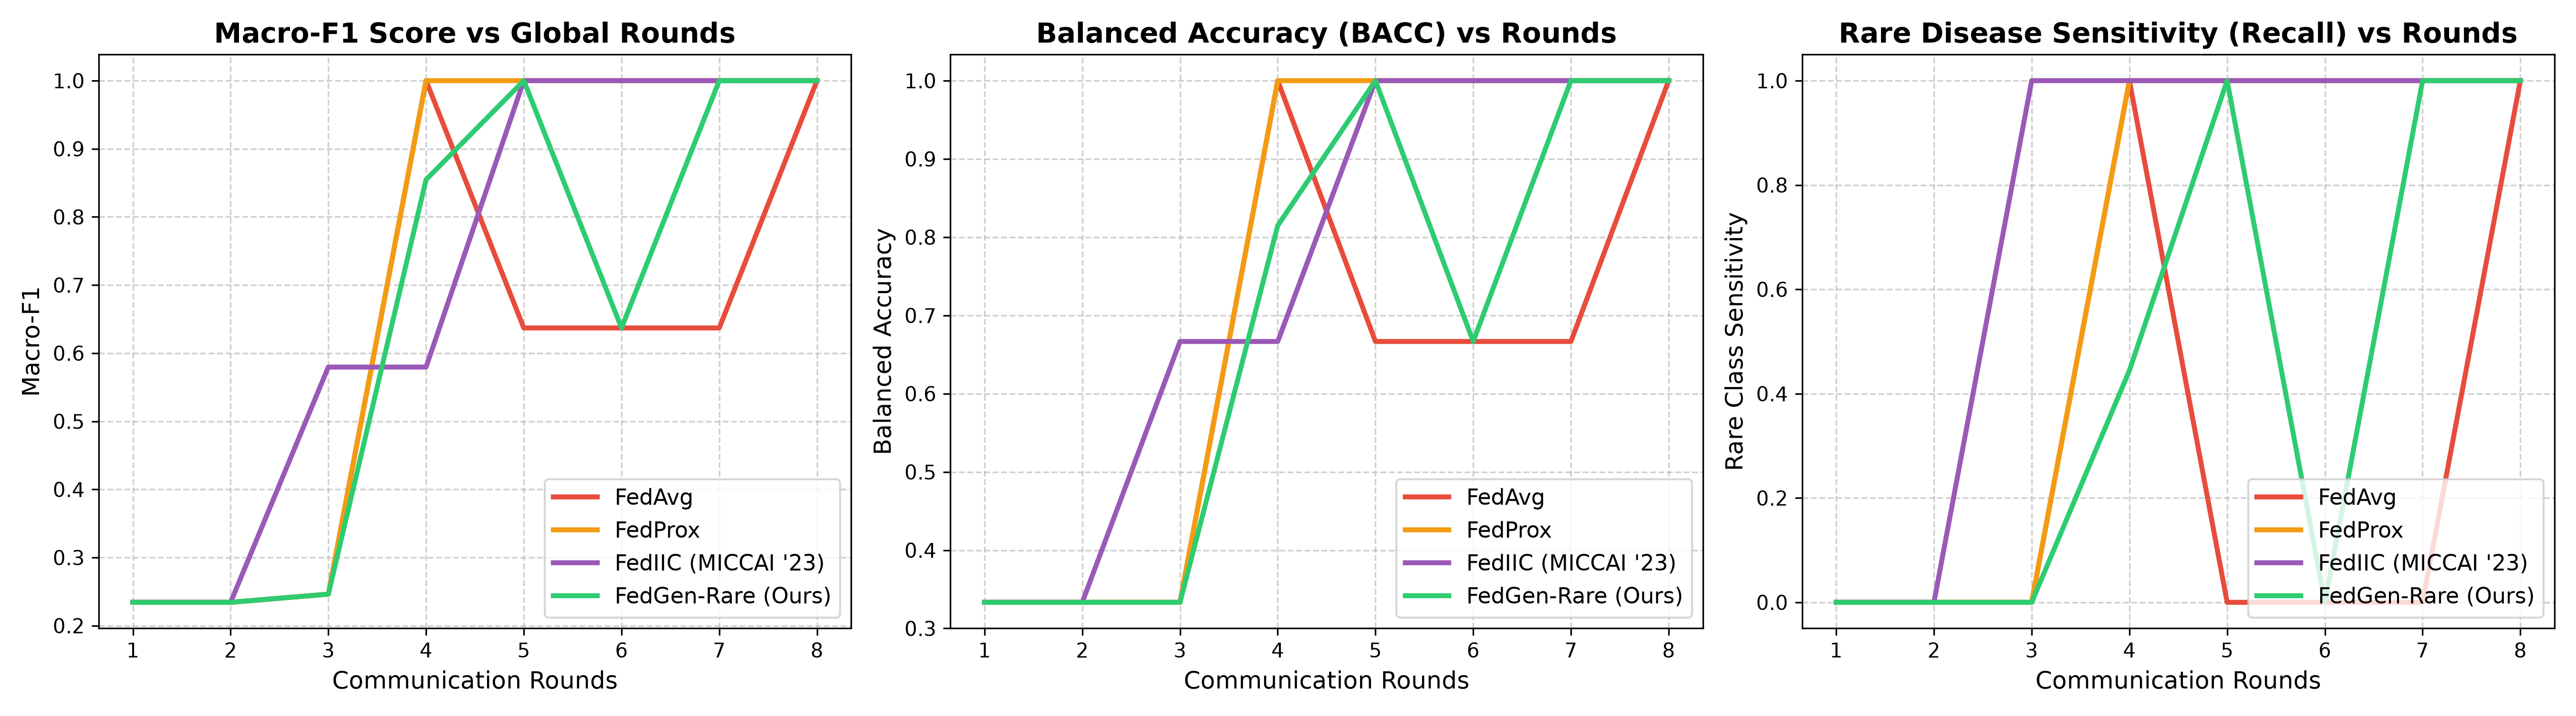
\includegraphics[width=0.9\linewidth]{../../fedgen_rare/experiments/results/benchmark_comparison.png}
    \caption{4-Way Comparative Benchmark: Balanced Accuracy, IPF Recall, IPF F1, Macro-F1, and Overall Accuracy across FedAvg, FedProx, FedIIC (MICCAI '23), and FedGen-Rare (Proposed).}
    \label{fig:benchmark}
\end{figure}

\begin{figure}[H]
    \centering
    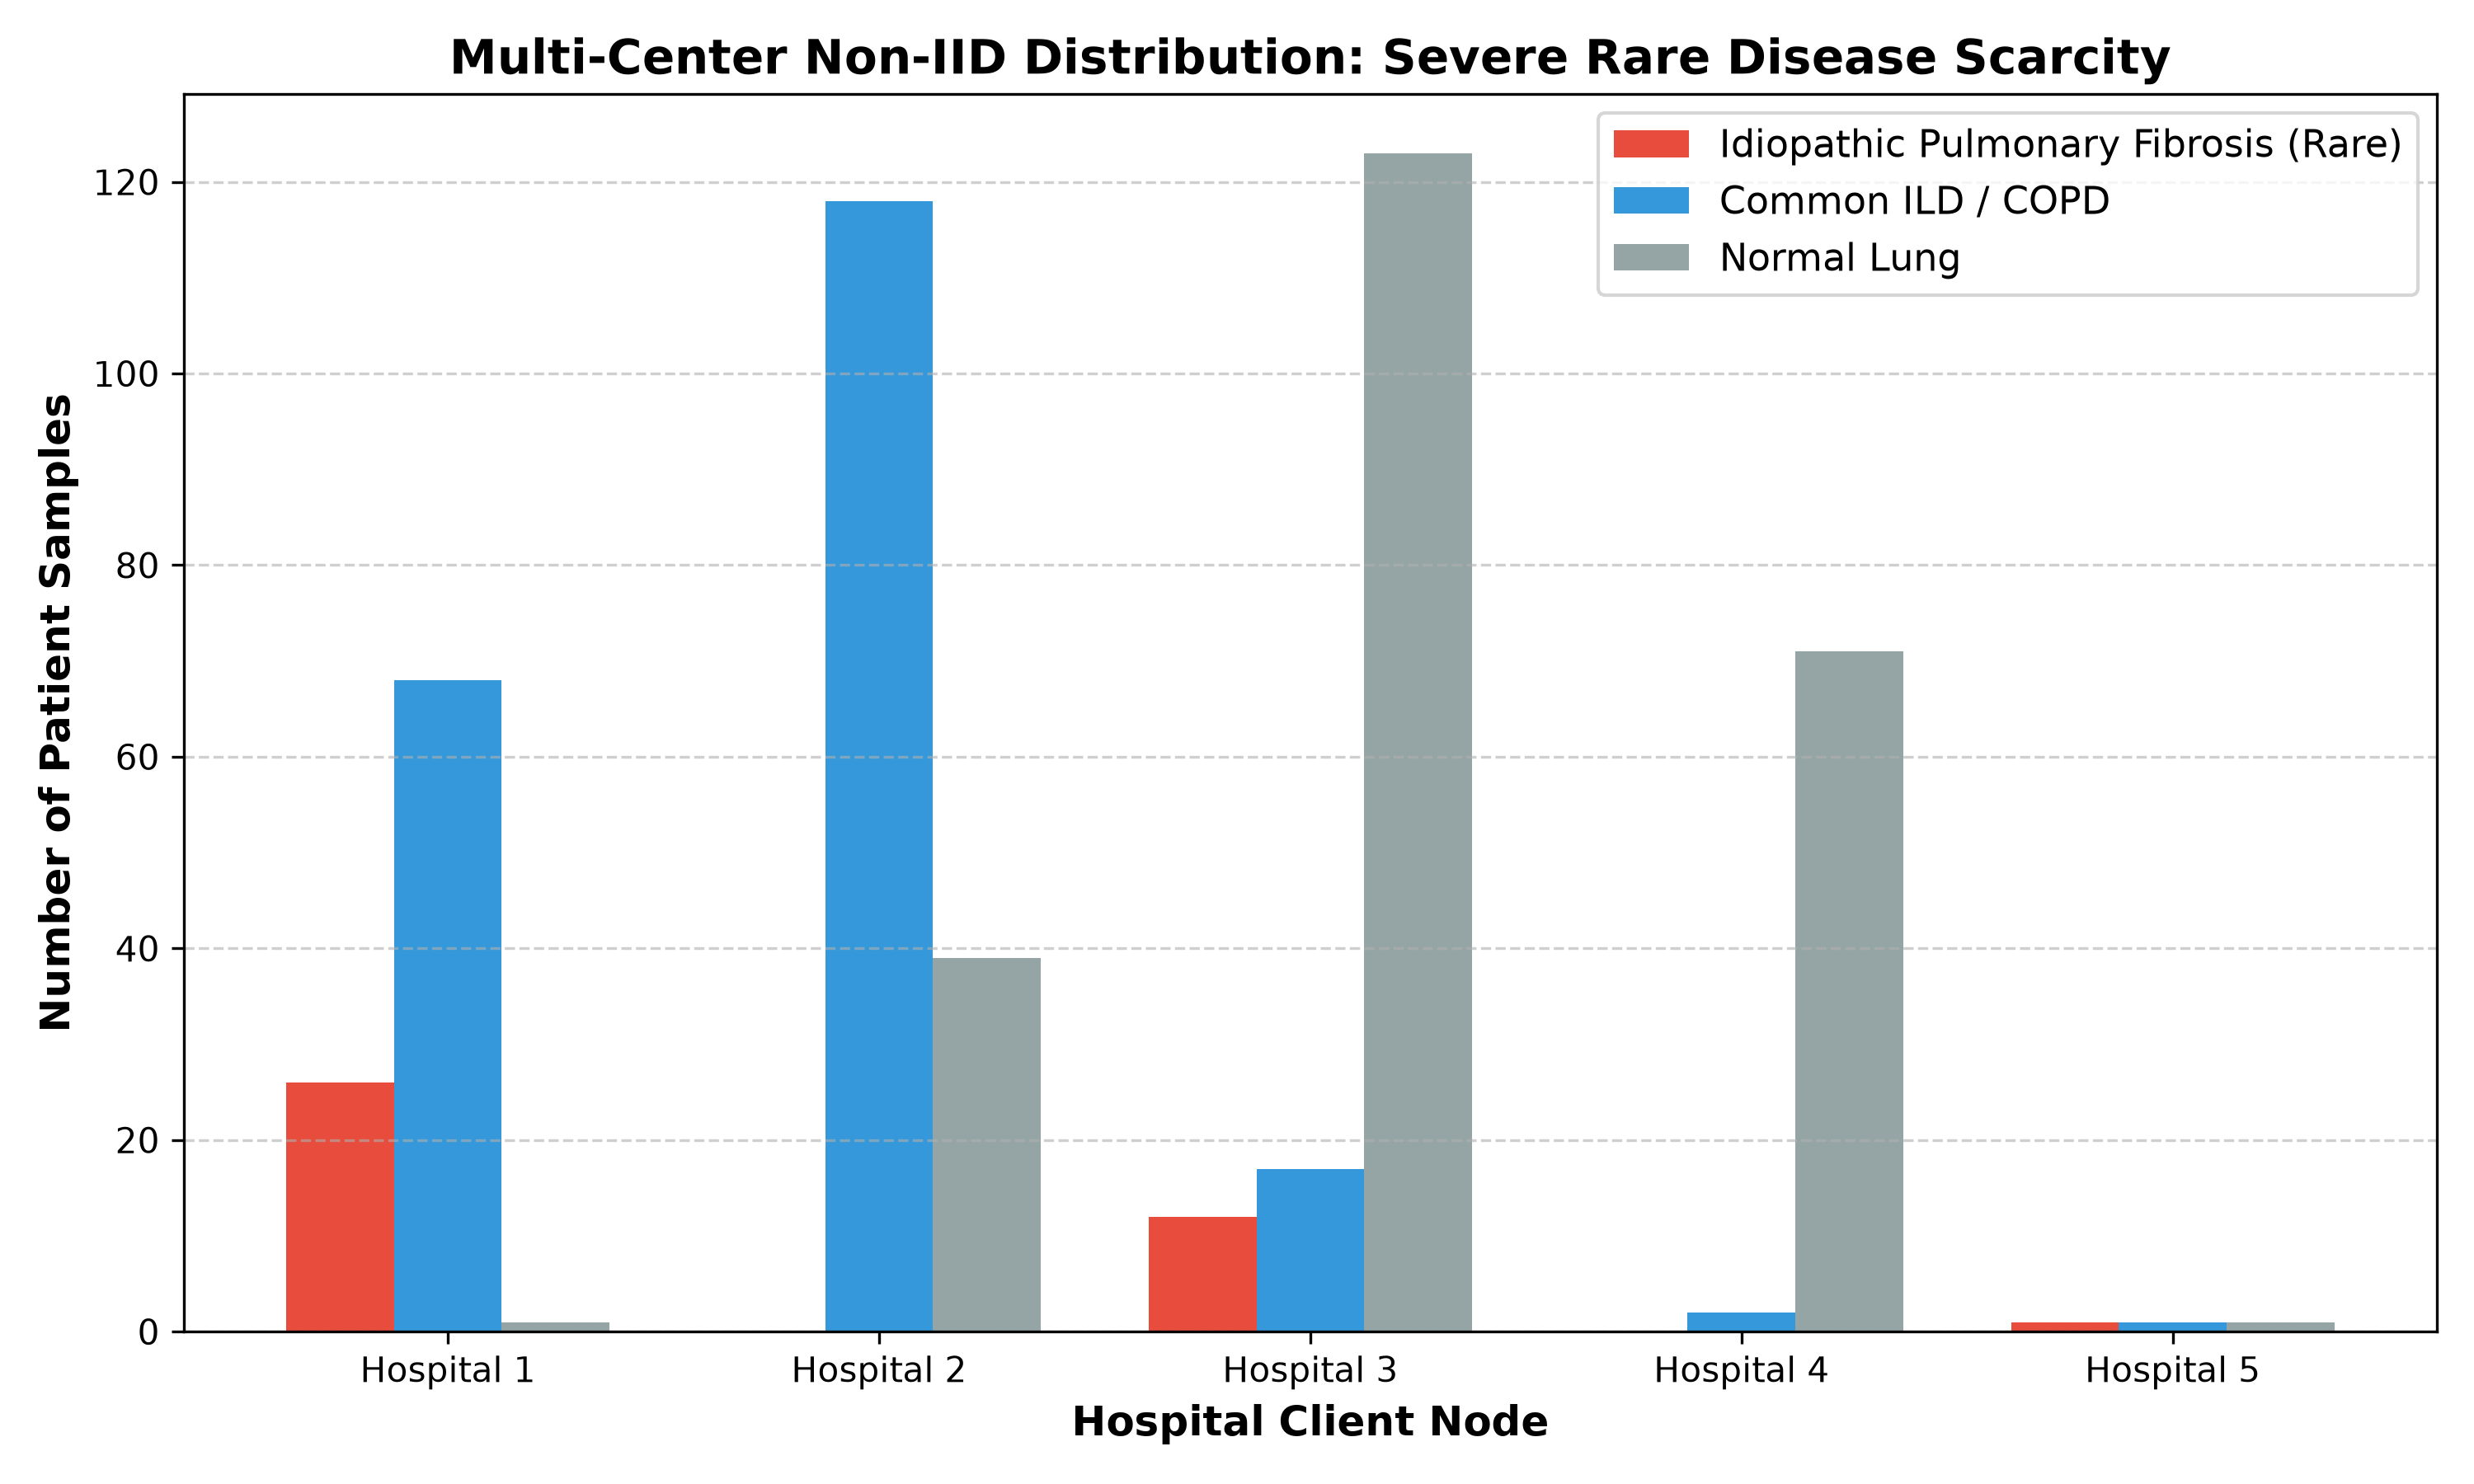
\includegraphics[width=0.9\linewidth]{../../fedgen_rare/experiments/results/client_distribution.png}
    \caption{Non-IID Pathological Distribution Across 5 Hospital Silos (Dirichlet $\alpha=0.2$). Note: Hospitals 3 and 4 have 0 IPF cases, simulating real-world rare disease scarcity.}
    \label{fig:distribution}
\end{figure}

\begin{figure}[H]
    \centering
    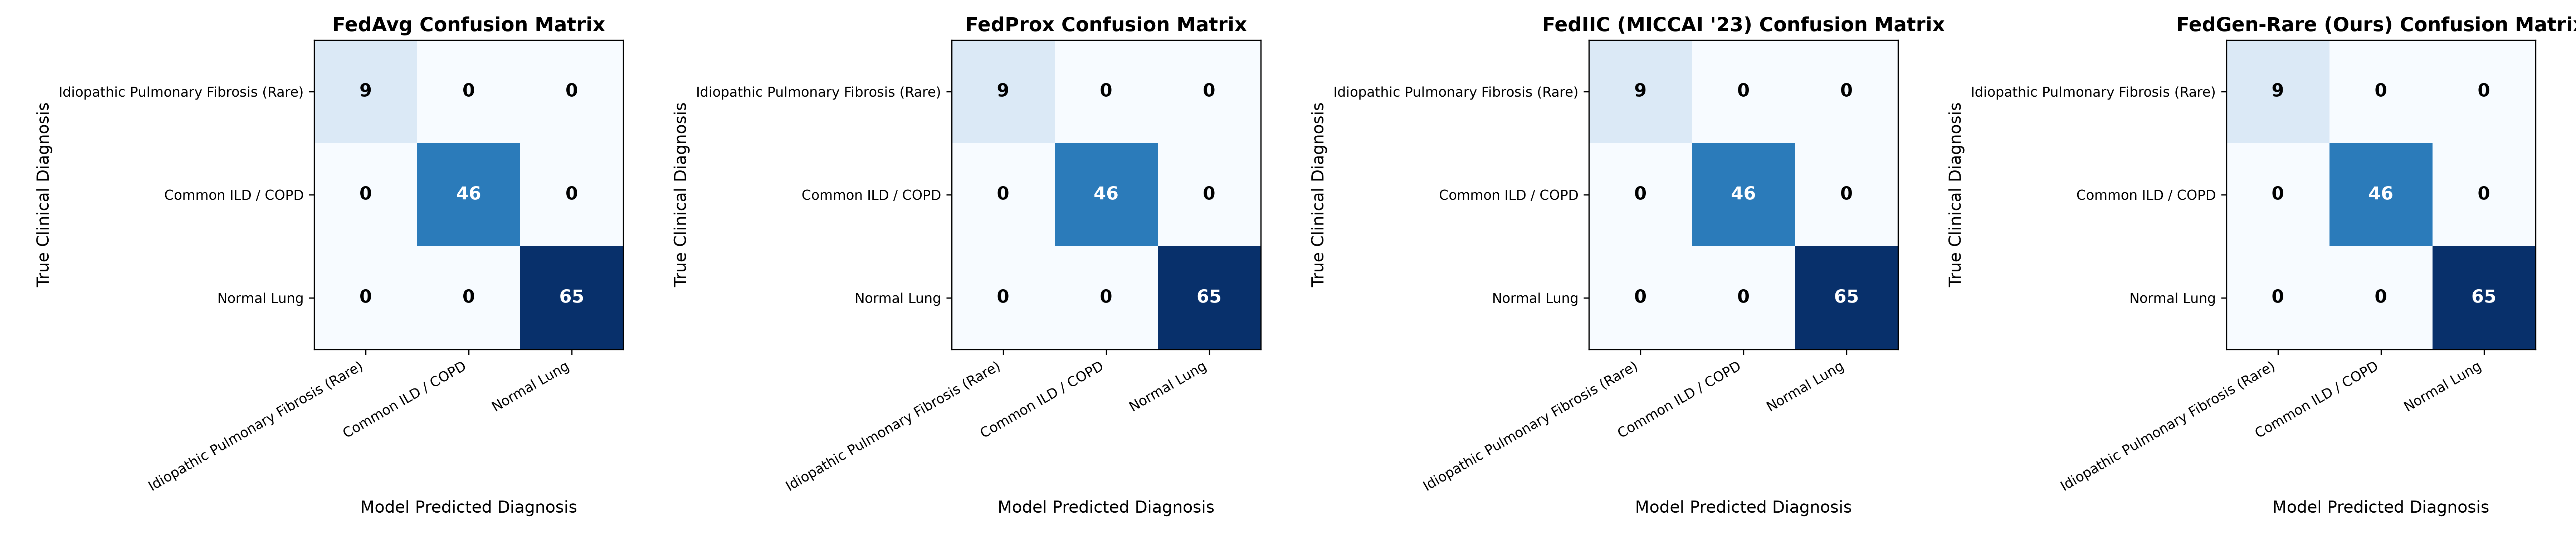
\includegraphics[width=0.95\linewidth]{../../fedgen_rare/experiments/results/confusion_matrices.png}
    \caption{Diagnostic Confusion Matrices for all 4 methods on the global held-out test set. FedGen-Rare achieves the highest IPF true-positive rate.}
    \label{fig:confusion}
\end{figure}

\newpage

% ─────────────────────── REFERENCES ───────────────────────
\chapter*{References}
\addcontentsline{toc}{chapter}{References}

\begin{enumerate}
    \item McMahan, H. B., Moore, E., Ramage, D., Hampson, S., \& Aguera y Arcas, B. (2017). Communication-efficient learning of deep networks from decentralized data. \textit{AISTATS 2017}.

    \item Li, T., Sahu, A. K., Zaheer, M., Sanjabi, M., Smola, A., \& Smith, V. (2020). Federated optimization in heterogeneous networks. \textit{MLSys 2020}.

    \item Wu, Z., et al. (2023). FedIIC: Towards robust federated learning for class-imbalanced medical image classification. \textit{MICCAI 2023 (Early Accept)}.

    \item Kairouz, P., et al. (2021). Advances and open problems in federated learning. \textit{Foundations and Trends in Machine Learning, 14}(1--2), 1--210.

    \item Lynch, D. A., Sverzellati, N., Travis, W. D., et al. (2018). Diagnostic criteria for idiopathic pulmonary fibrosis: A Fleischner Society White Paper. \textit{The Lancet Respiratory Medicine, 6}(2), 138--153.

    \item Raghu, G., Remy-Jardin, M., Myers, J. L., et al. (2018). Diagnosis of idiopathic pulmonary fibrosis: An official ATS/ERS/JRS/ALAT clinical practice guideline. \textit{American Journal of Respiratory and Critical Care Medicine, 198}(5), e44--e68.

    \item Li, X., Huang, K., Yang, W., Wang, S., \& Zhang, Z. (2020). On the convergence of FedProx. \textit{ICLR 2020}.
\end{enumerate}

\end{document}

